\subsubsection{Utente che utilizza lo smartphone per accedere alla dashboard}
\begin{wrapfigure}{l}{7cm}
    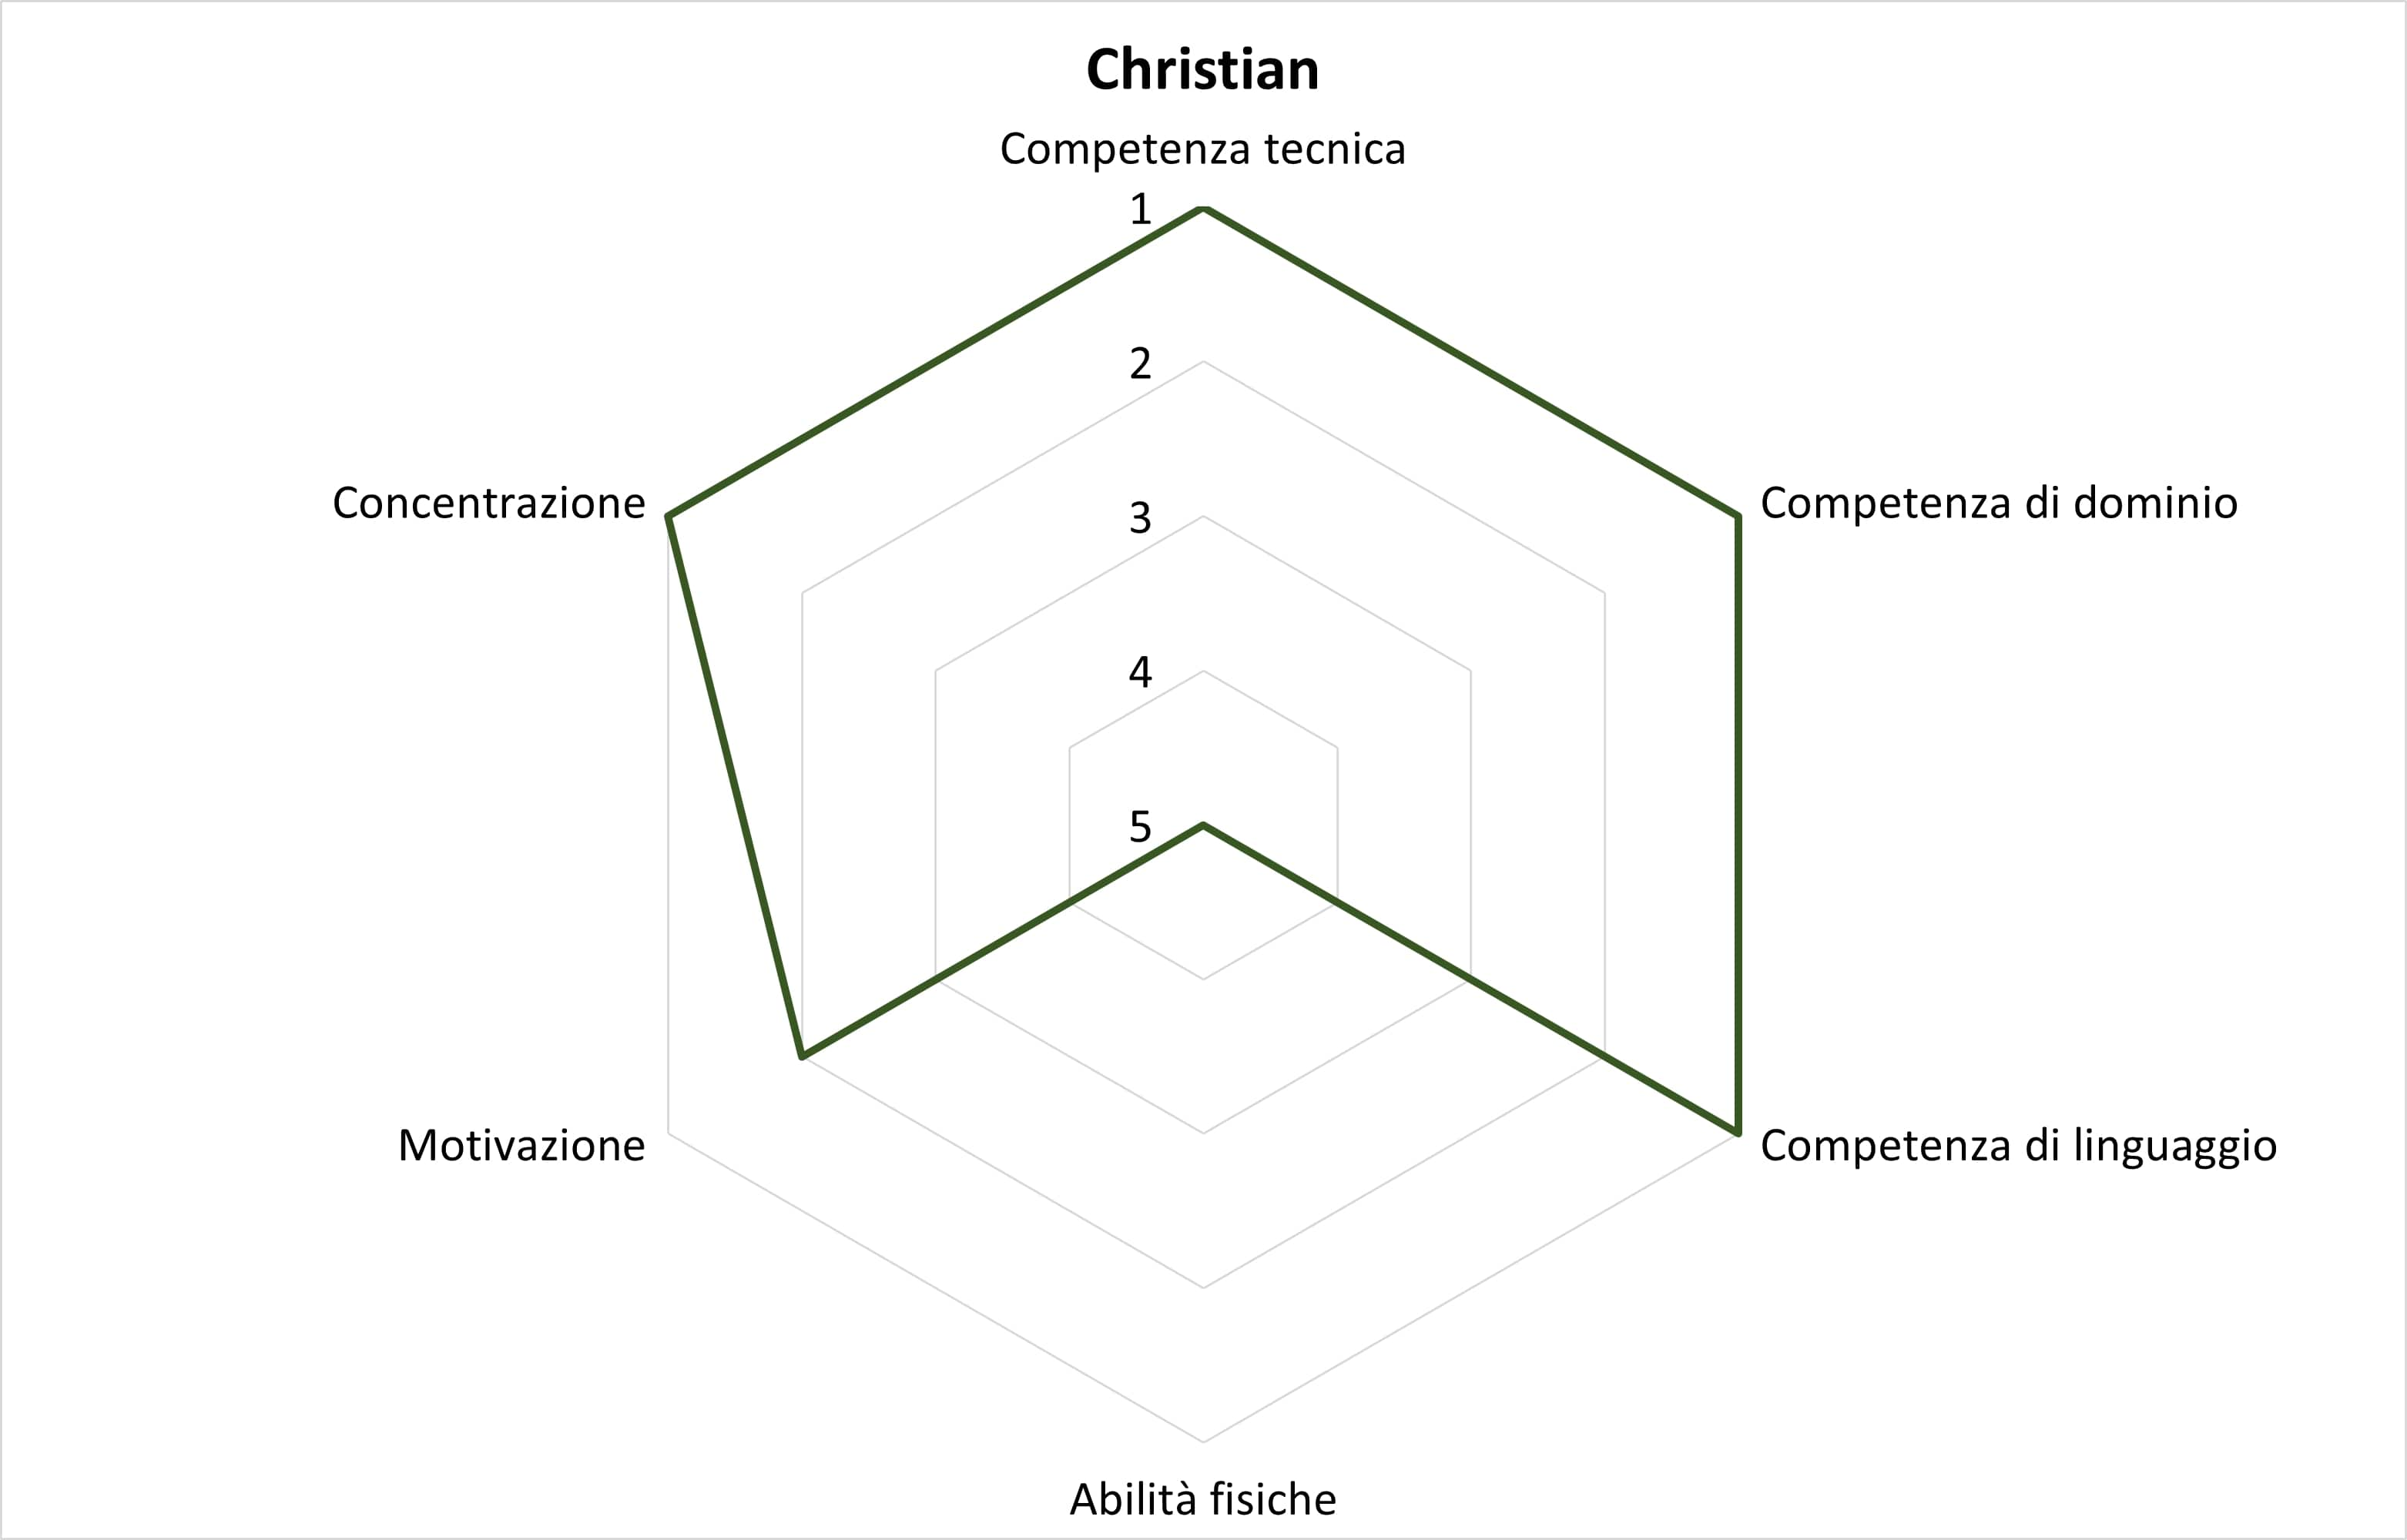
\includegraphics[scale=0.2]{studio-fattibilità/christian}
    \caption{Foto fantasiosa della persona Christian}
\end{wrapfigure}
Christian è un uomo di 34 anni che lavora come fattorino per un'agenzia di logistica. Ha un appartamento a Torino vicino a una fermata della metropolitana e per raggiungere la propria sede di lavoro deve necessariamente prenderla quotidianamente. La sua giornata di lavoro inizia con la raccolta dei pacchi che consegnerà con uno dei furgoni dell'azienda. Le restrizioni imposte alla mobilità delle persone dai vari DPCM ha aumentato notevolmente i clienti dei negozi online e di conseguenza il lavoro di Christian ne ha risentito parecchio. Al ritorno a casa, la sera, non gli avanza molto tempo libero in quanto vive da solo e deve provvedere anche alle faccende di casa. Inoltre, la stanchezza lo porta a desiderare di andare a dormire quanto prima, magari dopo essersi un po' riposato sul suo divano.\\
Nonostante il poco tempo a disposizione, vuole essere informato su ciò che avviene intorno a sé. Al mattino, prendendo la metropolitana, e in pausa pranzo, ascolta le rassegne stampa e legge alcuni giornali che ritiene affidabili, tra cui il \textit{Corriere della Sera}, attraverso il suo smartphone con uno schermo da 6''. Se gli capita, legge anche il bollettino che l'\textit{ANSA} ha pubblicato il giorno prima e che riporta i dati aggiornati sull'andamento dell'epidemia.
% \vspace{-5mm}
\begin{itemize}
	\item Attitudine:
    \begin{itemize}
        \item vita frenetica;
        \item non dedica un momento della propria routine all'informarsi in maniera sistematica dal computer;
    \end{itemize}
    \item Comportamento: si informa tramite le rassegne stampa;
    \item Obiettivi (\textit{end goals}): fare ipotesi sulle successive evoluzioni del Covid-19 e sui futuri provvedimenti governativi;
    \item Motivazione (\textit{life goals}): informarsi sommariamente su quel che sta accadendo;
    \item Obiettivi del sistema:
    \begin{itemize}
        \item segnalazione per l'utente che la fruizione è possibile esclusivamente in modalità desktop: tramite dispositivo mobile dallo schermo contenuto, l'esperienza utente sarebbe eccessivamente limitata. 
    \end{itemize}
\end{itemize}